\documentclass[12pt, a4paper]{ctexart}

\usepackage{fancyhdr}
\pagestyle{fancy}
\fancyhead{}
\renewcommand{\headrulewidth}{1pt}
\renewcommand{\headwidth}{\textwidth}
\fancyhead[L]{北京大学基础物理实验报告}
\fancyhead[R]{\thepage}
\fancyfoot{}

\fancypagestyle{plain}{
\fancyhead{}
\renewcommand{\headrulewidth}{1pt}
\fancyfoot{}
\fancyhead[C]{北京大学基础物理实验报告}
}
\usepackage[colorlinks,linkcolor=red,urlcolor = blue]{hyperref}
\usepackage{booktabs}
\usepackage{graphicx}
\usepackage{amsmath}
\usepackage{mathcomp}
\usepackage{mathabx}
\usepackage{enumitem}
\usepackage[top=1.2in, bottom=1.2in, left=1in, right=1in]{geometry}
\usepackage{array}
\usepackage{tabularx}
\newcolumntype{C}{>{\centering\arraybackslash}X}
\usepackage{subfig}
\usepackage{wrapfig}
\usepackage{textcomp}
\usepackage{abstract}
\usepackage[backend=bibtex]{biblatex}



\ctexset{
    section={   
        name={,},
        number={\chinese{section}},
        format=\heiti\raggedright
    },
    subsection={   
        name={(,)},
        number={\chinese{subsection}},
        format=\heiti
    }
}

\begin{document}
\title{基于虚拟仪器的电路综合实验}
\date{2024年9月}

\maketitle
\tableofcontents
\clearpage

\section{实验I:用虚拟仪器测量电阻的伏安特性}

\subsection*{仪器用具}
计算机(含操作系统)、LabVIEW 2020,数据采集卡,$100\Omega$标准电阻,待测电阻$R_1 = 1k\Omega$
和$R_2 = 50\Omega$各一个,导线若干。

\subsection{实验原理}
见实验讲义。

\subsection{实验数据}

\begin{figure}[!h]
    \centering
    \subfloat[$R_1^{(1)}$]{
        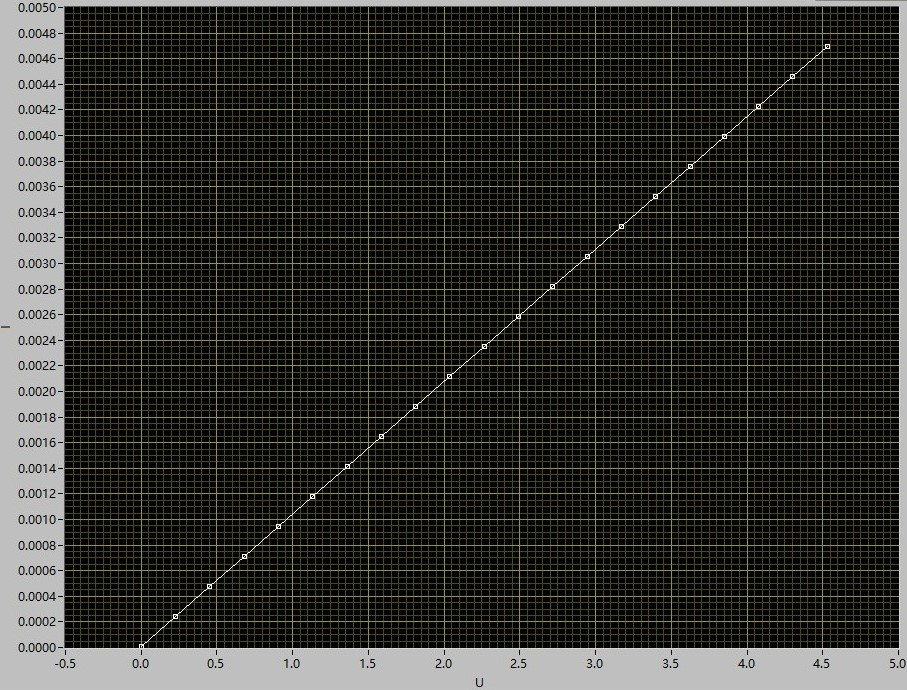
\includegraphics[width=0.45\linewidth]{./figure/U-I_1kOmega(1).jpg}
        }\hfill
    \subfloat[$R_1^{(2)}$]{
        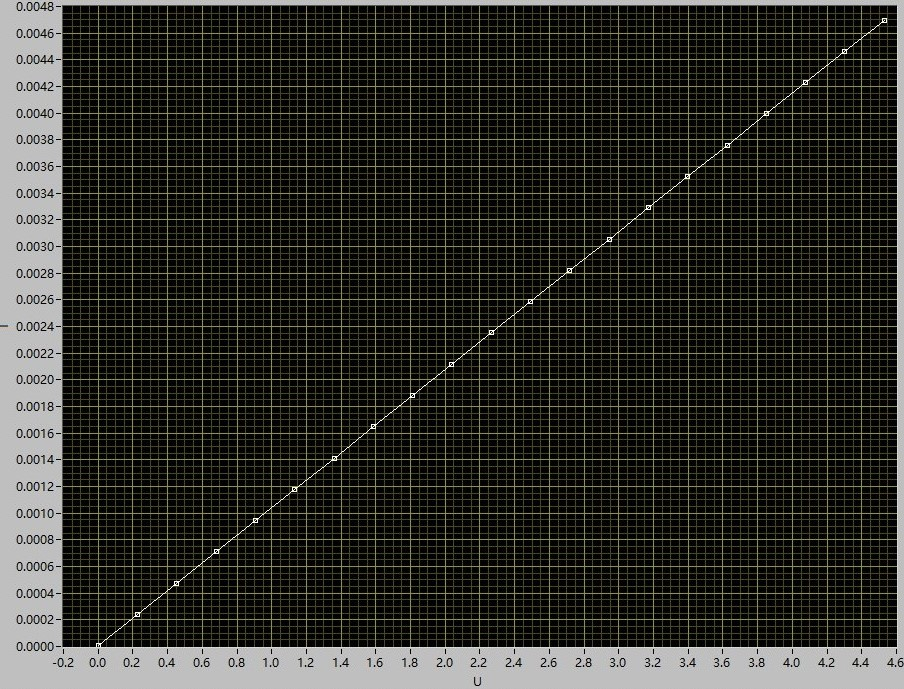
\includegraphics[width=0.45\linewidth]{./figure/U-I_1kOmega(2).jpg}
        }

    \subfloat[$R_1^{(3)}$]{
        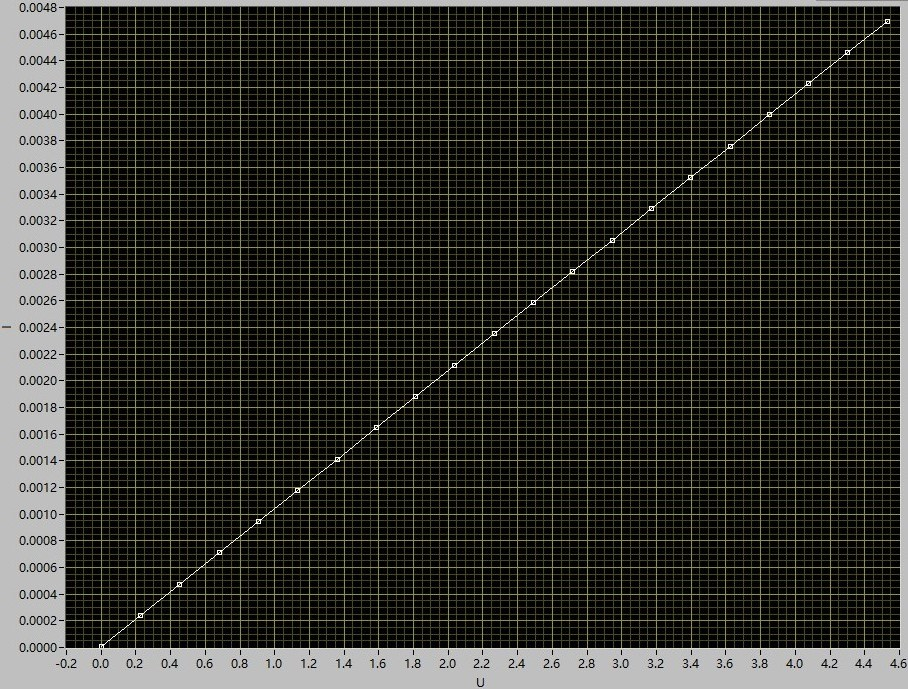
\includegraphics[width=0.45\linewidth]{./figure/U-I_1kOmega(3).jpg}
        }\hfill
    \subfloat[$R_2^{(1)}$]{
        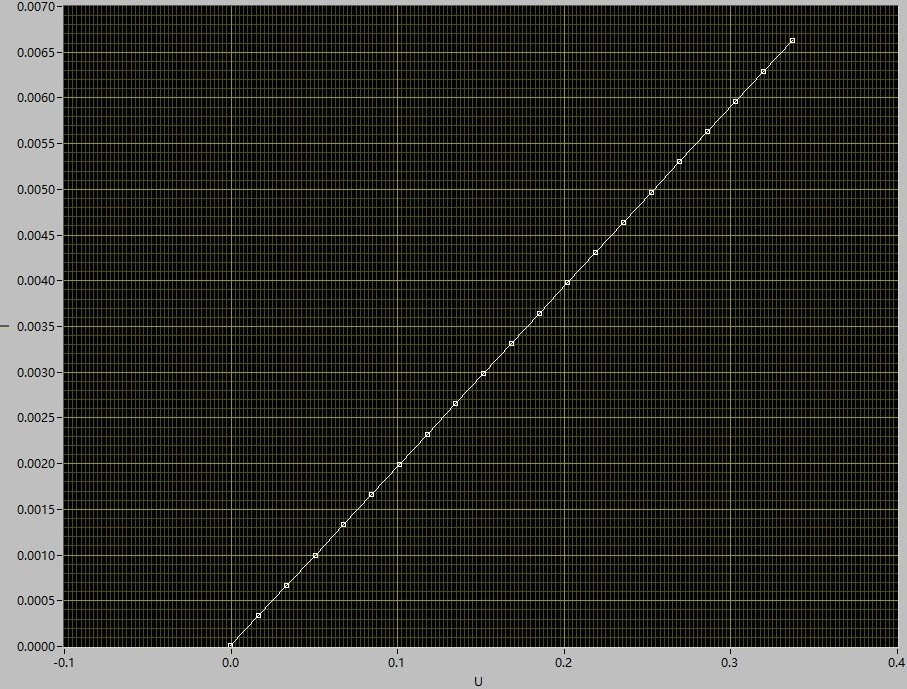
\includegraphics[width=0.45\linewidth]{./figure/U-I_50Omega(1).jpg}
        }

    \subfloat[$R_2^{(2)}$]{
        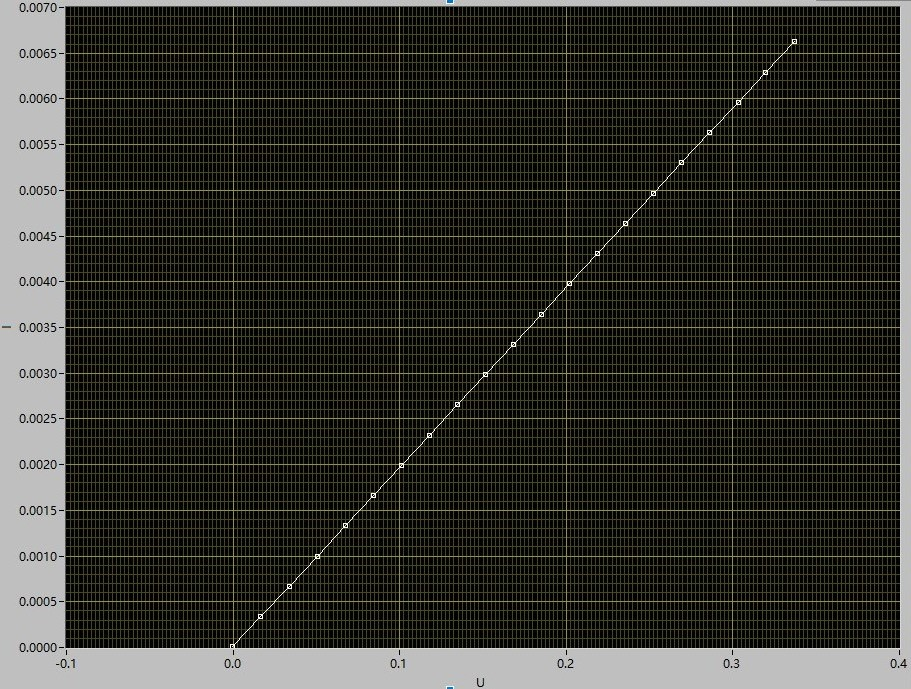
\includegraphics[width=0.45\linewidth]{./figure/U-I_50Omega(2).jpg}
        }\hfill
    \subfloat[$R_2^{(3)}$]{
        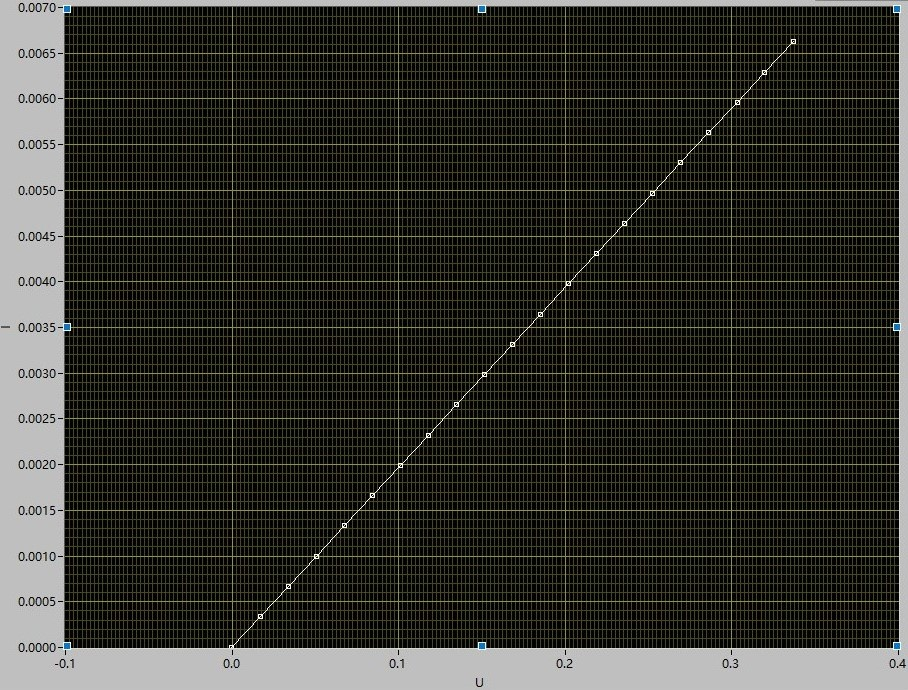
\includegraphics[width=0.45\linewidth]{./figure/U-I_50Omega(3).jpg}
        }
    \caption{虚拟仪器测得的待测电阻的伏安特性曲线}
    \label{fig:1}
\end{figure}


图\ref{fig:1}(a)-(c)为标称值$1k\Omega$电阻的测量结果,图\ref{fig:1}(d)-(f)为标称值$50\Omega$电阻的测量结果,电阻实际测量值为图斜率倒数,由程序自动计算得到,见表\ref{tab:1}。

\begin{table}[!h]
    \centering
	\caption{虚拟仪器得到的电阻测量值}
	\begin{tabularx}{.55\textwidth}{C|ccc}
	\toprule
	序号$i$ & 1 & 2 & 3 \\
	\midrule
	$R_{1i}$实测值/$\Omega$ & 965.540 & 965.502 & 965.457 \\
	$R_{2i}$实测值/$\Omega$ & 50.8808 & 50.8760 & 50.8738 \\
	\bottomrule
	\end{tabularx}
    \label{tab:1}
\end{table}

\subsection{实验结果}

对测量得到的结果进行简单计算可以得到待测电阻值:
\begin{gather*}
    R_1 = \frac{1}{3} \sum_{i = 1}^{3} R_{1i} = 965.500 \Omega\\
    R_2 = \frac{1}{3} \sum_{i = 1}^{3} R_{2i} = 50.8769 \Omega
\end{gather*}

鉴于虚拟仪器的特点以及最终收集的有效数据,该实验不进行多余的误差分析。

\section{实验II:稳压二极管正反向伏安特性曲线测量}

\subsection{仪器用具}

除实验I中提到的仪器外,将待测电阻改为稳压二极管。
程序框图与实验I中没有太多差异(个人水平和实验时间有限,没有用LabVIEW程序写出相应的正反向电压测量语句)。

\begin{figure}[!h]
    \centering
    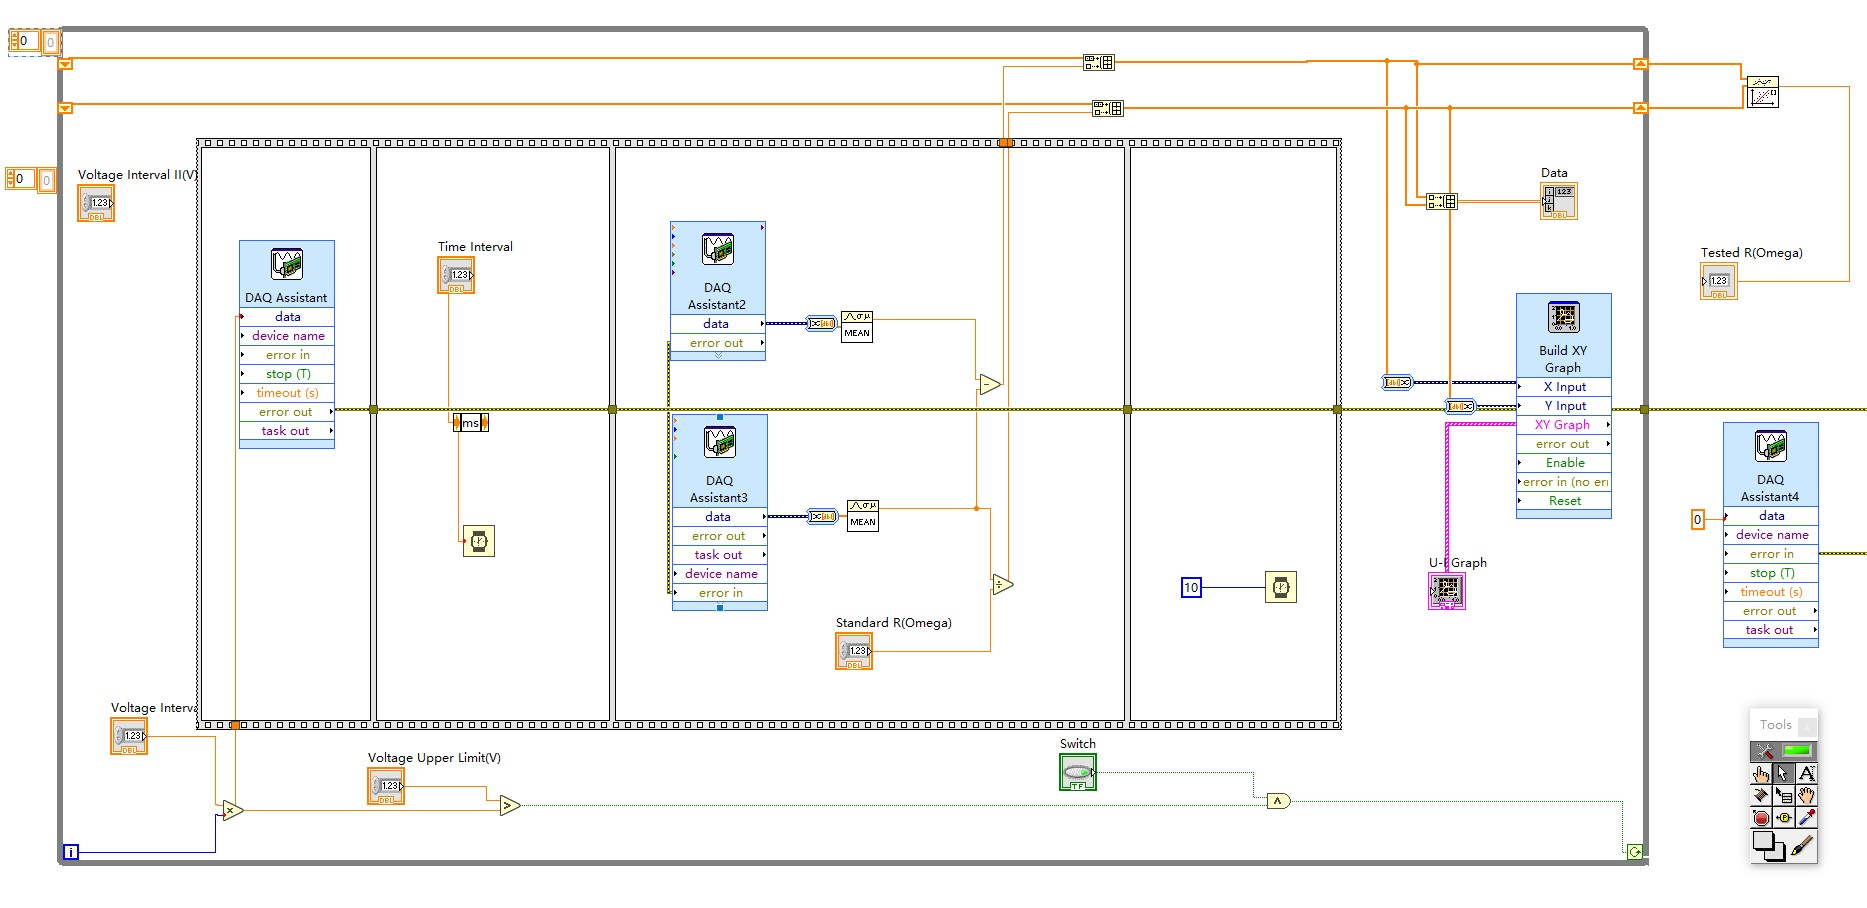
\includegraphics[width=5in]{./figure/Block Diagram(U-I).jpg}
    \caption{程序框图}
\end{figure}

\begin{figure}[!h]
    \centering
    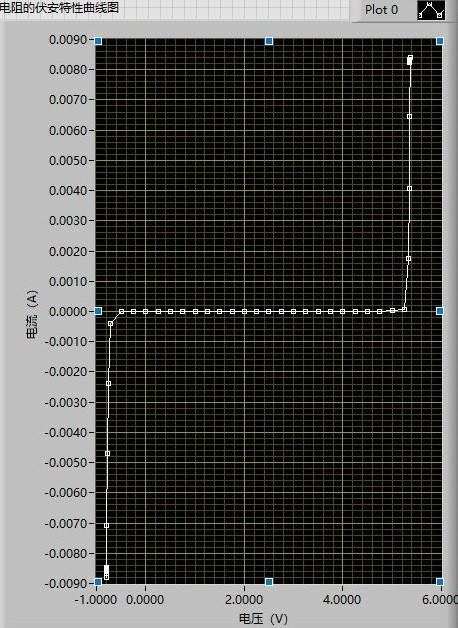
\includegraphics[width=3in]{./figure/Diode.jpg}
    \caption{二极管正反向伏安特性曲线}
    \label{fig:2}
\end{figure}

\subsection{实验结果}

根据\ref{fig:2}展示的数据,可以得到:
\begin{itemize}
    \item $I_1 = 4mA$时,$U_1 = 5.34V$,静态电阻值为$R_{st}(4mA) = \frac{U_1}{I_1} = 1.3k\Omega$。
    \item $I_2 = -4mA$时,$U_2 = -0.79V$, 静态电阻为$R_{st}(-4mA) = \frac{U_1}{I_1} =0.2k\Omega$。
\end{itemize}

数据较为粗略,故不作误差分析。

\section{实验III:Fano共振}

\subsection{仪器用具}

计算机(含操作系统)、LabVIEW 2020,数据采集卡,电阻箱一个($0.1-100k\Omega$),电容箱两个($0.0001-1\mu F$),标称$100\Omega$电阻一个,标称18mH、16mH电感各一个,标称$0.047\mu F$电容一个,信号发生器。

\subsection{理论推导}

Fano共振是对传统共振现象的重要补充和拓展,该现象在很多物理体系中普遍存在。
本题研究的是在双RLC耦合电路中出现的一种Fano共振现象。

\begin{wrapfigure}{l}{2.5in}
    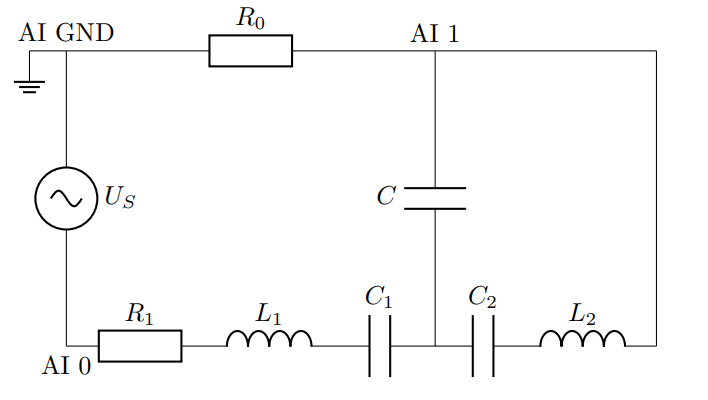
\includegraphics[width=2.5in]{figure/Fano_circuiTikz.png}
    \caption{实验电路}
    \label{fig:3}
\end{wrapfigure}

如左图所示,两耦合RLC电路系统中两电路利用共用电容C形成耦合,电路中的电容、电感等元件均为非理想元件,将两电路中分别存在的额外损耗记为$r_1$,$r_2$,
设电容$C_1$右侧极板带电量为$q_1$,电容$C_2$左侧极板带电量为$q_2$,则由电荷守恒得电容$C$上极板带电量为$q_1 + q_2$,我们可以列出回路方程:

\begin{align}
    L_1 \frac{d^2 q_1}{dt_2} + (R_0 + R_1 + r_1) \frac{dq_1}{dt} + \frac{q_1}{C_1} + \frac{q_1 + q_2}{C} &= U_S e^{i\omega t}\\
    L_2 \frac{d^2 q_2}{dt_2} + r_2 \frac{dq_2}{dt} + \frac{q_2}{C_2} + \frac{q_1 + q_2}{C} &= 0
\end{align}

化简后可得
\begin{align}
    \ddot{q_1} + \gamma_1 \dot{q_1} + \omega_1 q_1 + g_{12}q_2 &= a_1 e^{i\omega t}\\
    \ddot{q_2} + \gamma_2 \dot{q_2} + \omega_2 q_2 + g_{12}q_1 &= 0
\end{align}
其中
\begin{gather*}
    \omega_1^2 = \frac{1}{L_1}(\frac{1}{C_1} + \frac{1}{C}),\quad \omega_2^2 = \frac{1}{L_2}(\frac{1}{C_2} + \frac{1}{C})\\
    \gamma_1 = \frac{R_0 + R_1 + r_1}{L_1},\quad \gamma_2 = \frac{r_2}{L_2},\quad g_{12}^2 = \frac{1}{C^2 L_1 L_2}
\end{gather*}
代入试探解
\begin{equation}
    q_1 = q_{10}e^{i\omega t}\quad q_2 = q_{20}e^{i\omega t}
\end{equation}
可以得到$q_1$,$q_2$的振幅为
\begin{align}
    q_{10} &= \frac{(\omega_2^2 - \omega^2 + i\gamma_2 \omega)}{(\omega_1^2 - \omega^2 + i\gamma_1 \omega)(\omega_2^2 - \omega^2 + i\gamma_2 \omega) - g_{12}^2}a_1\\
    q_{20} &= -\frac{g_{12}}{(\omega_1^2 - \omega^2 + i\gamma_1 \omega)(\omega_2^2 - \omega^2 + i\gamma_2 \omega) - g_{12}^2}a_1
\end{align}
相应相位定义为
\begin{equation}
    q_{10}(\omega) = |q_{10}(\omega)|e^{-i\phi (\omega)}, \quad q_{20}(\omega) = |q_{20}(\omega)|e^{-i\phi_2 (\omega)}
\end{equation}
其中二者相位差
\begin{equation*}
    \phi_2 - \phi = \pi - \theta
\end{equation*}
而$\theta$由下式给出
\begin{equation}
    \theta = \tan^{-1}\Big(\frac{\gamma_2 \omega}{\omega_2^2 - \omega^2}\Big)
\end{equation}
待测部分为$AI 0$与$AI 1$之间的电路,相应参数下标为x,即
\begin{equation*}
    U_x e^{i\phi_x} = U_S e^{i\omega t} - R_0 \frac{dq_1}{dt}
\end{equation*}

当系统1损耗较大(对应宽谱共振),系统2损耗较小(对应窄谱共振),且耦合系数$g_{12}$具有合适的数值时,耦合体系可以发生显著的Fano共振现象:
此时,系统1的响应谱在系统2的谐振频率$\omega_2$附近会出现非对称的Fano共振线型(表现为一个非对称的共振峰,区别于对称的洛伦兹线型),参考文献[1][2]。

\subsection{实验数据}

\subsubsection{电容电感参数表征}

调试参数前,我们先使用实验室提供的电容电感表征程序测量了电容和电感的复阻抗,结果如图\ref{fig:4}。
\begin{figure}
    \centering
    \subfloat[标称值18mH电感]{
        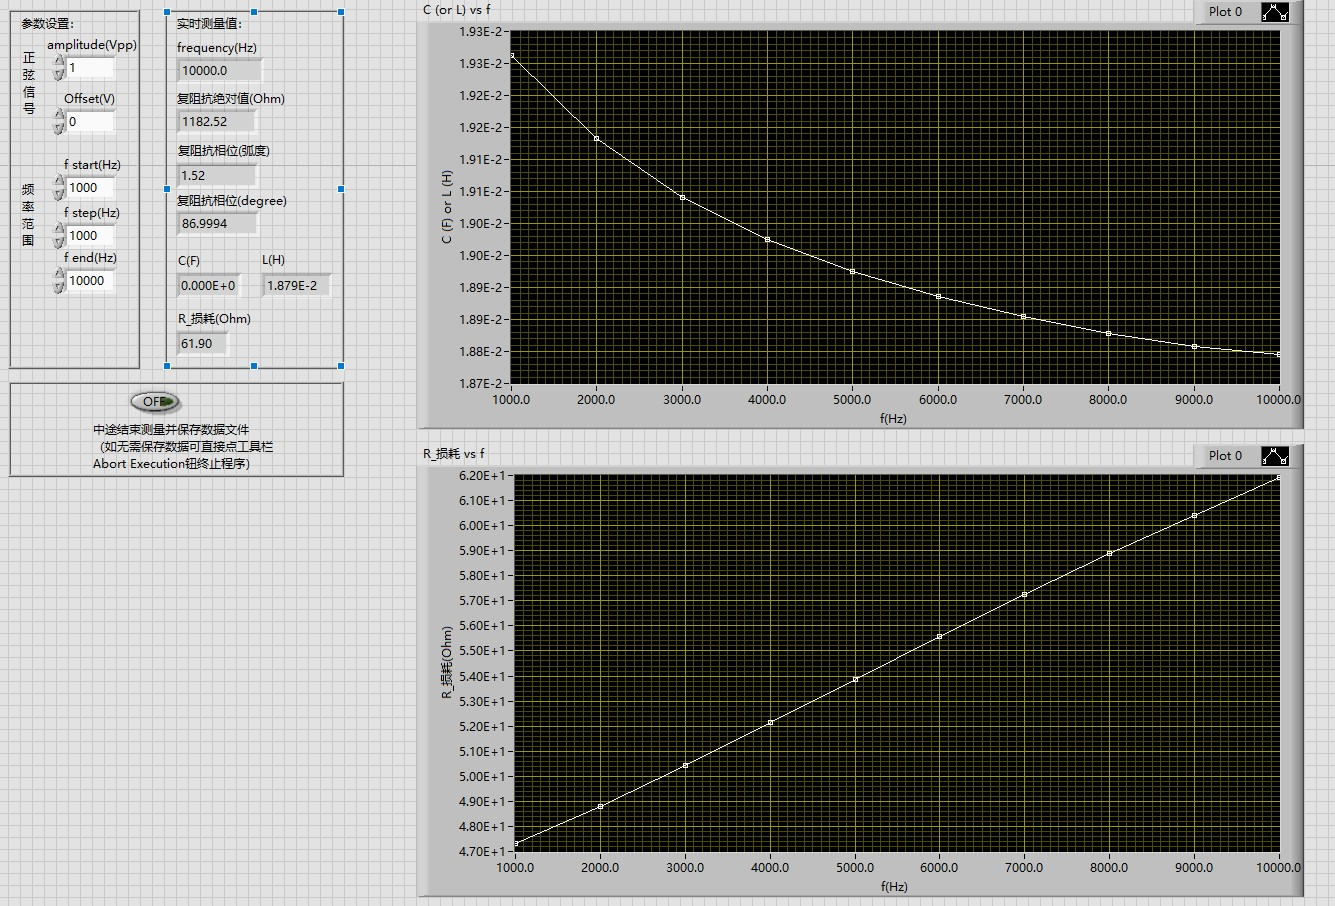
\includegraphics[width=0.7\linewidth]{./figure/18mH.jpg}
        }

    \vspace{-0.1in}
    \subfloat[标称值16mH电感]{
        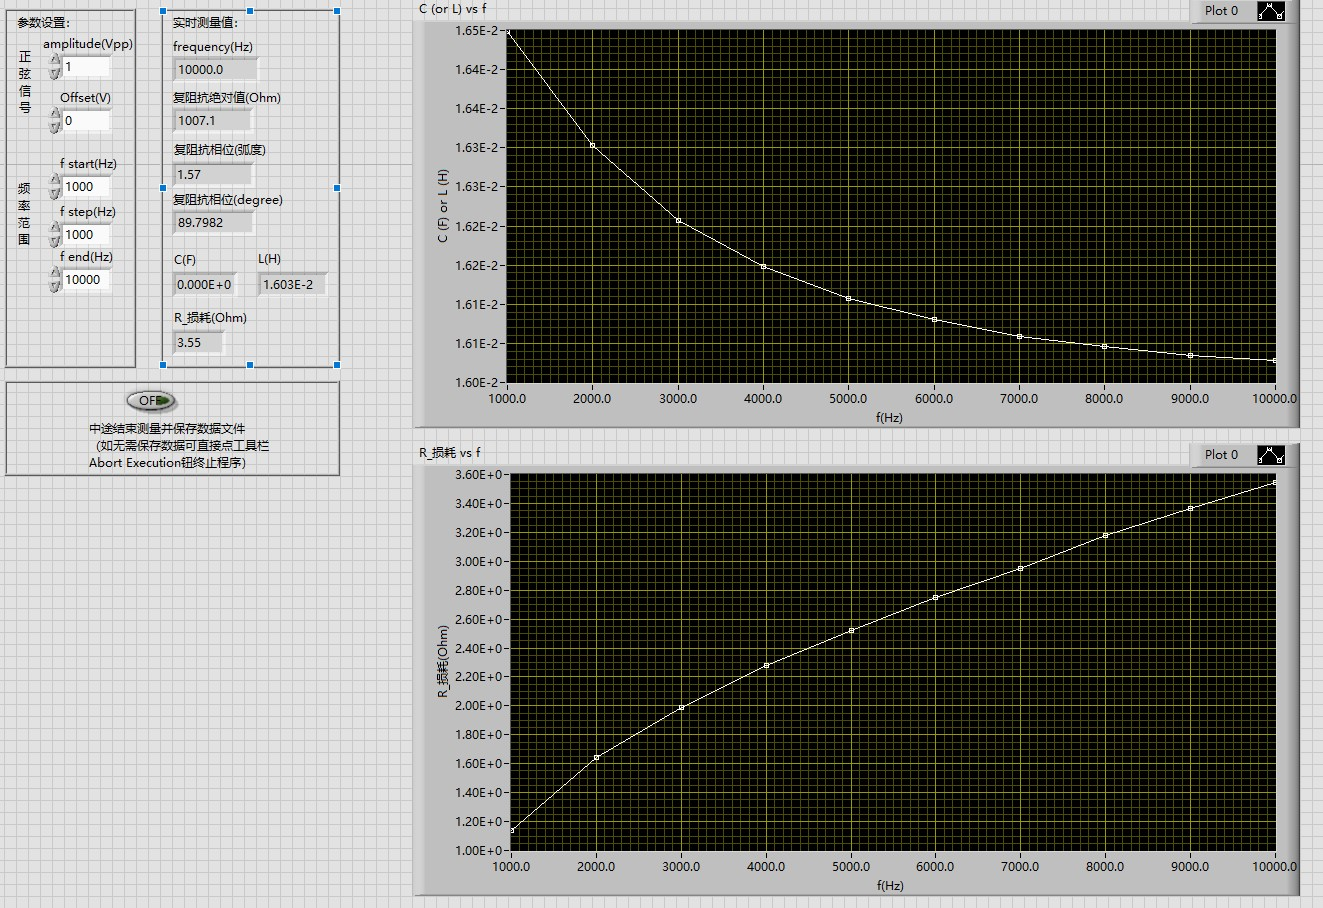
\includegraphics[width=0.7\linewidth]{./figure/16mH.jpg}
        }

    \vspace{-0.1in}
    \subfloat[标称值0.047$\mu F$电容]{
        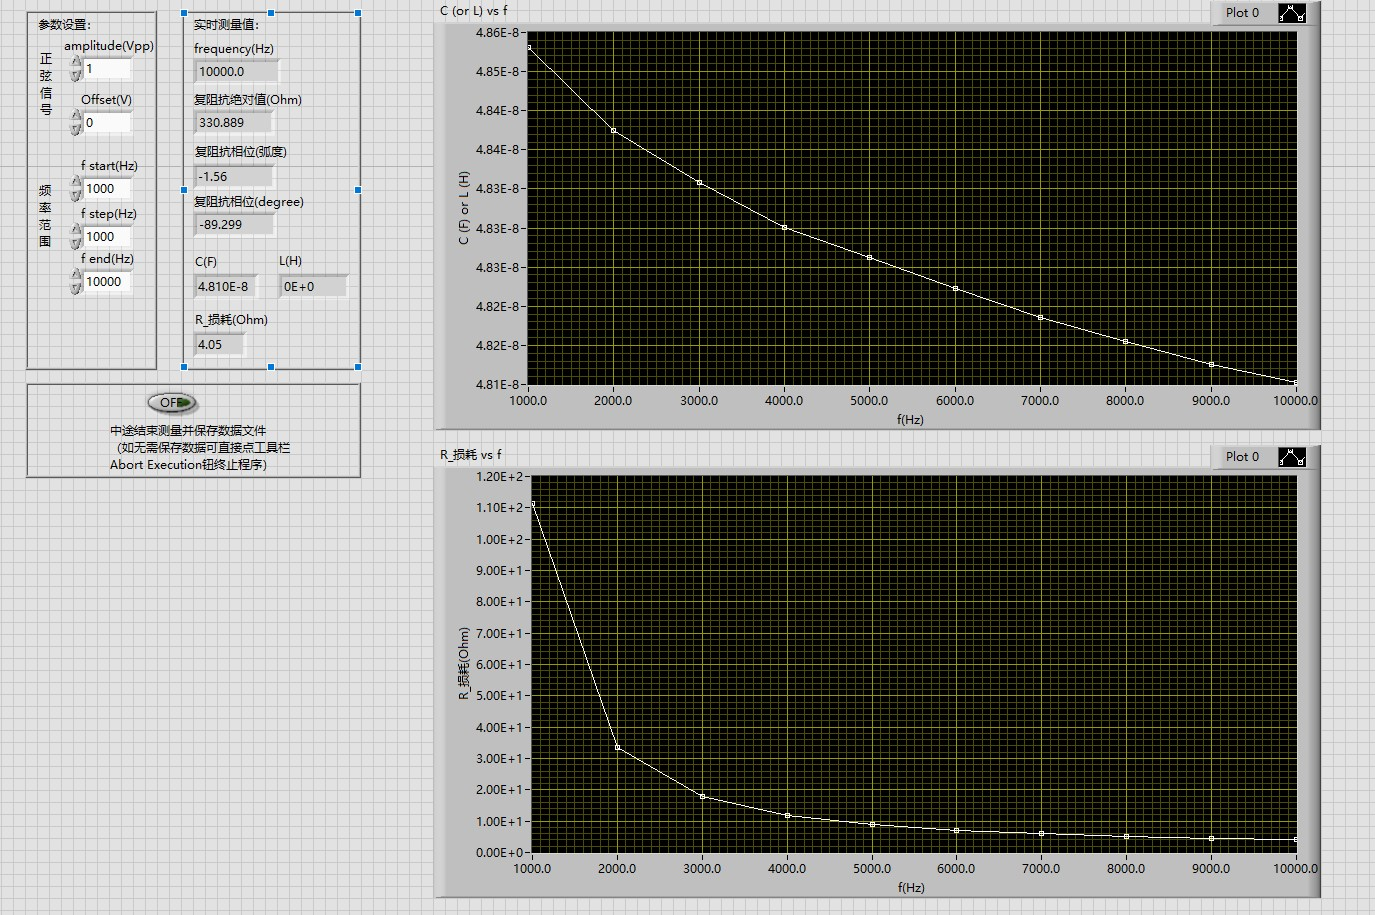
\includegraphics[width=0.7\linewidth]{./figure/0.047uF.jpg}
        }
    \caption{电容电感表征结果}
    \label{fig:4}
\end{figure}

从程序前面板显示的数据中可以看出,各元件的感抗(容抗)都基本在标称值的合理误差范围内,但两电感的损耗电阻存在较大差异:
16mH电感的损耗电阻仅在$\sim 1\Omega$的数量级,但18mH电感的损耗电阻大致为$\sim 50\Omega$的数量级,明显大于前者。
而0.047$\mu F$电容的损耗电阻在2000Hz以上的较高频段下大致处于$\sim 10\Omega$的数量级。
故在估计$r_1$、$r_2$以及调节参数时应考虑这些元件损耗电阻的影响。

\subsubsection{标准参数下的Fano共振}

为实现Fano共振,要求$\gamma_1$较大而$\gamma_2$较小。
由前面的理论推导可以得到,在当前实验条件下需要较大的$R_1$来增大系统1的耗散系数,同时在系统1中使用耗散较高的18mH电感。
同时为较为清晰地观察到Fano共振产生的非对称峰,要求$\omega_1$与$\omega_2$的间距较大,即增大图像中两峰的距离,这就要求$C_2 \gg C_1$。
通过简单的参数调节可以得到,当$L_1$使用18mH电感,$C_1$使用0.047$\mu F$电容,$R_1$使用500$\Omega$电阻箱,$L_2$使用16mH电感,$C_2$使用0.2$\mu F$电容器时能够观察到较为明显的Fano共振峰,测得的结果如图\ref{fig:5}所示。
\begin{figure}[!ht]
    \centering
    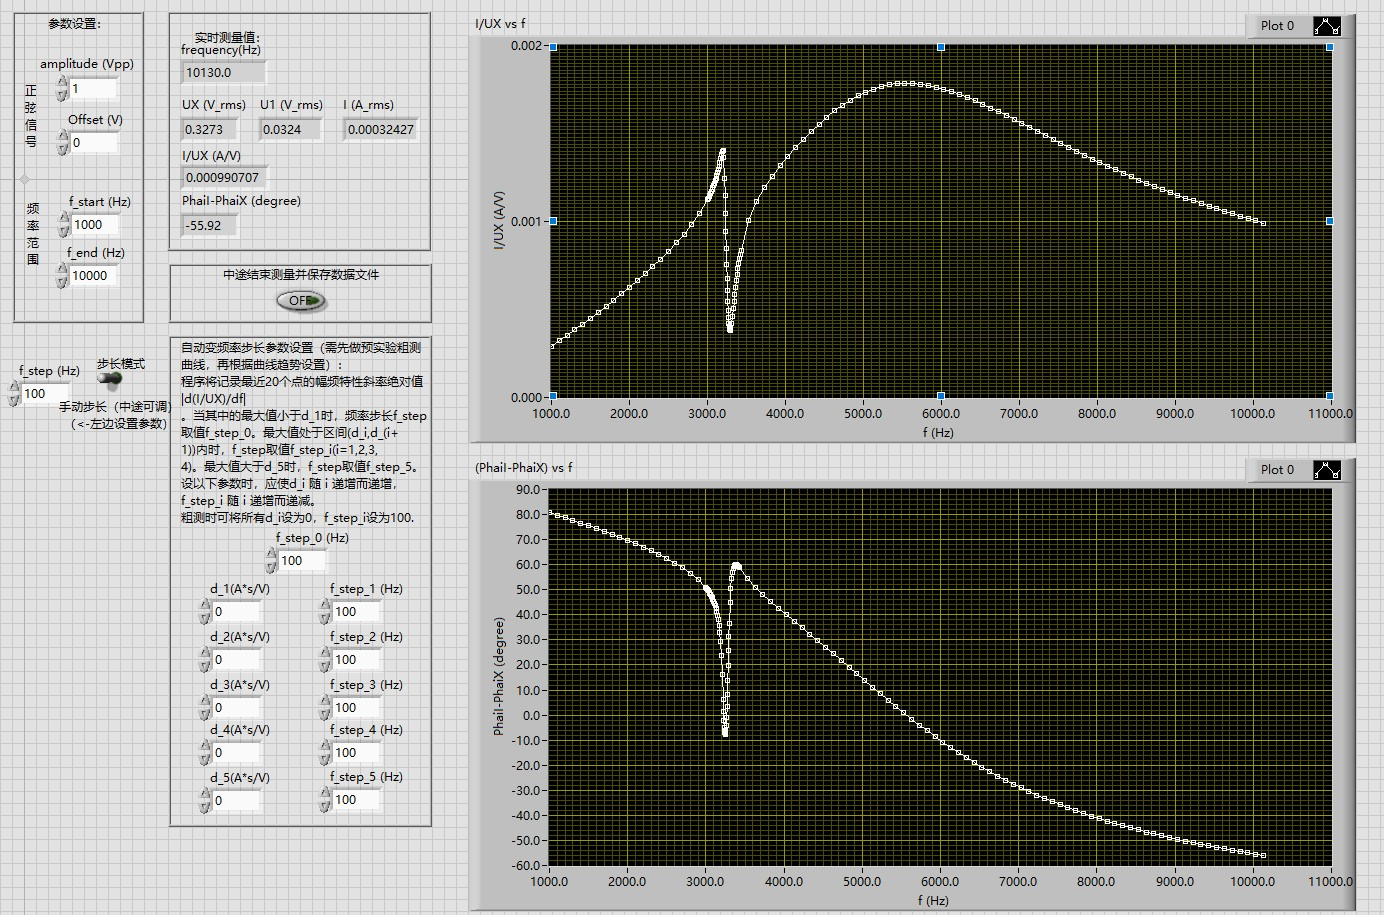
\includegraphics[width=0.8\linewidth]{./figure/standardFano.jpg}
    \caption{标准参数下的Fano共振图像}
    \label{fig:5}
\end{figure}

从图中可以看出,Fano共振峰处对应相位的谷,相反共振谷则对应相位峰,这是符合我们物理图像的预期的。
当输入相位和系统振动相位之差较大时,两矢量相加结果较小,而相应在相位谷处相位差接近0$^{\circ}$,两矢量几乎重合,此时达到共振,振幅为极大值。

\subsubsection{Fano共振特征随系统参数变化}

通过调整电路元件参数可以研究两系统中的损耗、耦合、谐振频率等参量对Fano共振现象的影响。
但由于电路元件的限制,只有$C$,$C_2$和$R_1$三个元件参数可供调节,其中$R_1$变化对应$\gamma_1$的改变,$C_2$变化对应$\omega_2$的改变,而$C$的变化会同时引起$\omega_1$和$\omega_2$的变化。

\begin{itemize}
    \item 调节$R_1$
\end{itemize}

\begin{figure}[!ht]
    \centering
    \subfloat[I/UX vs f Graph]{
        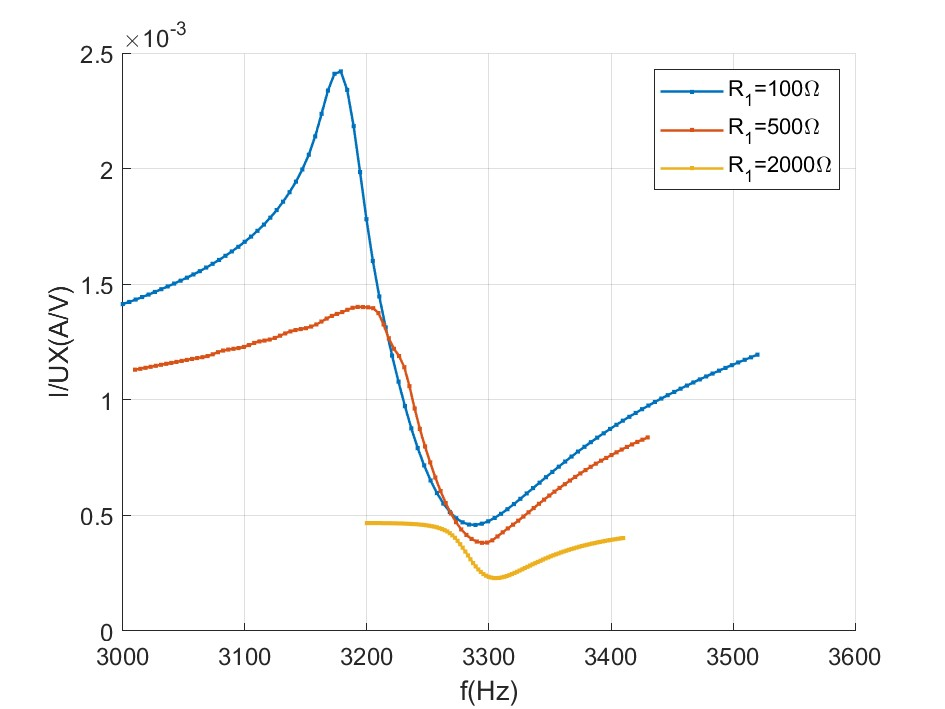
\includegraphics[width=0.5\linewidth]{./figure/Change_R1.jpg}
        \label{fig:5a}
        }
    \subfloat[$\phi -\phi_x$ vs f Graph]{
        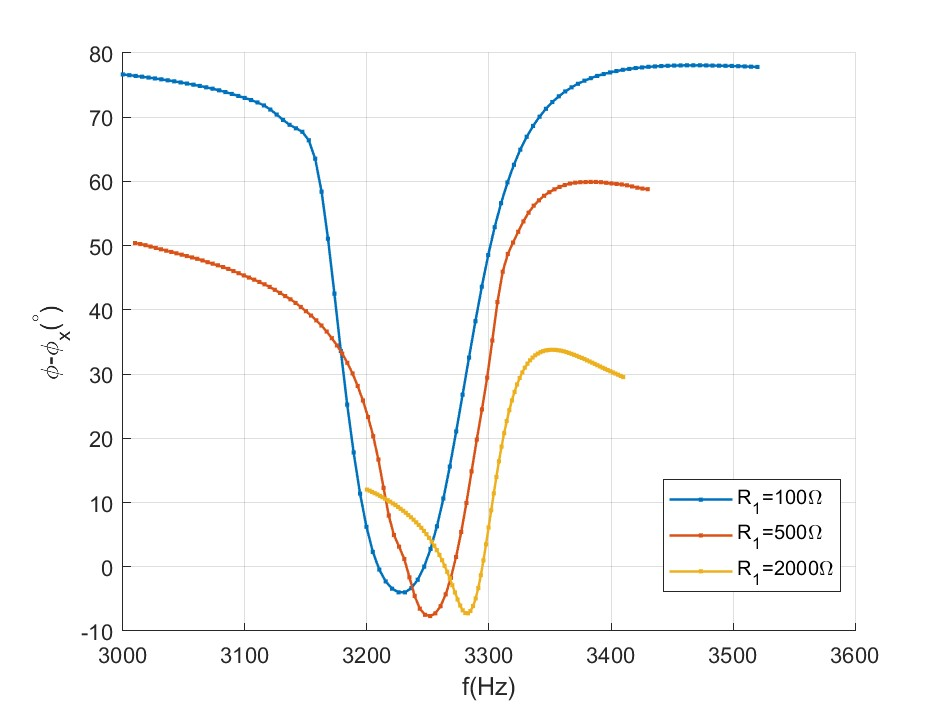
\includegraphics[width=0.5\linewidth]{./figure/phi-phi_x-R_1.jpg}
        \label{fig:5b}
    }
    \caption{不同$R_1$电路中的共振图像}

    \centering
    \subfloat[I/UX vs f Graph]{
        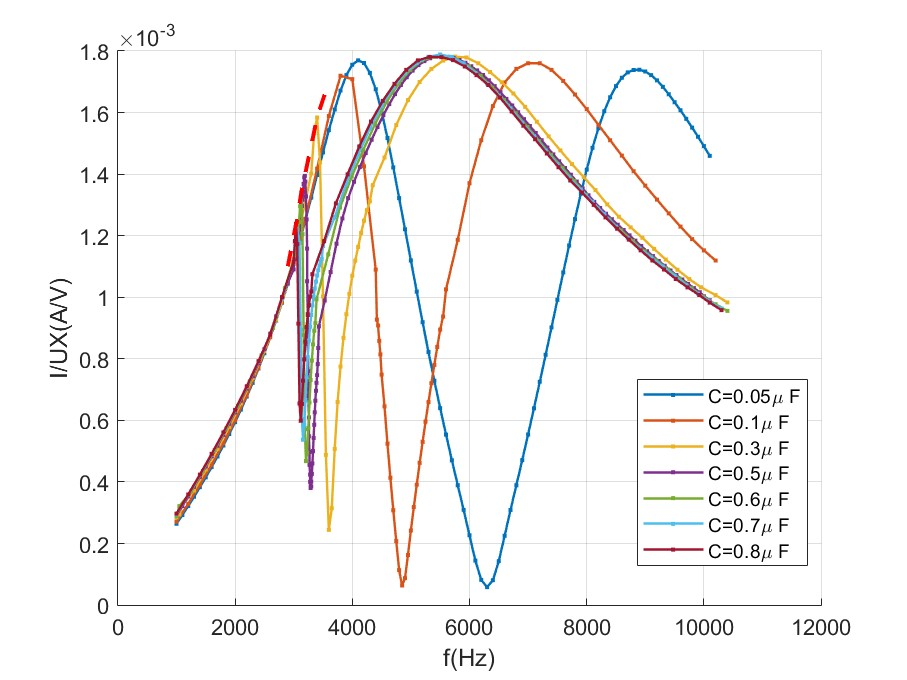
\includegraphics[width=0.5\linewidth]{./figure/Change_C.jpg}
        \label{fig:6a}
        }
    \subfloat[$\phi -\phi_x$ vs f Graph]{
        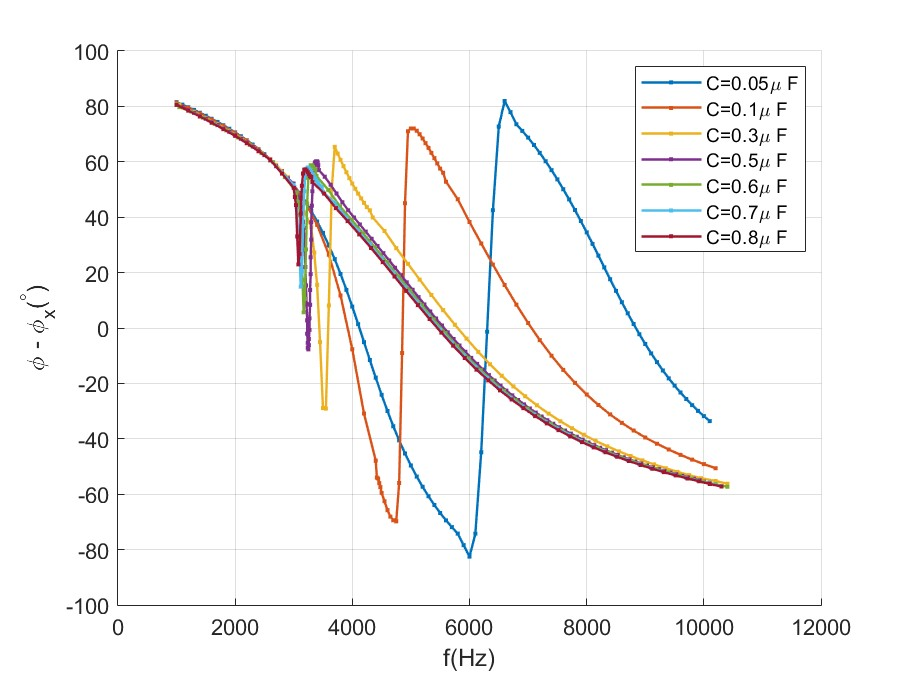
\includegraphics[width=0.5\linewidth]{./figure/phi-phi_x-C.jpg}
        \label{fig:6b}
    }
    \caption{不同$C$电路中的共振图像}
\end{figure}

从图\ref{fig:5a}中可以看出,随着$\gamma_1$即系统1损耗的增加,共振峰幅值不断减小,对应在图\ref{fig:5b}中即表现干路电流与待测部分电压相位差变化幅度的减小。
这样的变化与物理图像给出的直观是符合的比较好的,在此不作赘述。

另外可以看到共振峰位置随$R_1$增大呈现一个向高频移动的趋势,这和相位差受到$\gamma_1$的调制有关,相位差的谷位置也在随$R_1$增大向高频移动。
同时注意到相位差为0的位置与共振峰并不完全重合,这与我们选择的纵坐标有关。

\begin{itemize}
    \item 调节$C$
\end{itemize}

如图\ref{fig:6a},当$C$相对较大时(保证耦合系数$g_{12}$处于一个较为恰当的数量级),可以观察到较为明显的Fano共振现象;
但$C = 0.05\mu F$的条件下就呈现出两个洛伦兹线型的共振峰(相比标准情形耦合系数增大两个数量级)。
根据理论推导可以得到Fano共振峰应处于$\omega_2$对应频率处,用数量级大致估计得到$f_2 \sim 3000Hz$,实验数据与其符合程度较高。
图\ref{fig:6a}中的红色虚线即为共振峰位置随$C$的大致变化趋势(部分)。
由于$C$的变化导致的共振峰右移可由$\omega_2$的变化解释,而上移则主要是由于$g_{12}$改变导致的系统2振幅的增大和极小相位差向0的不断趋近。

\begin{itemize}
    \item 调节$C_2$
\end{itemize}

\begin{figure}[!t]
    \centering
    \subfloat[I/UX vs f Graph]{
        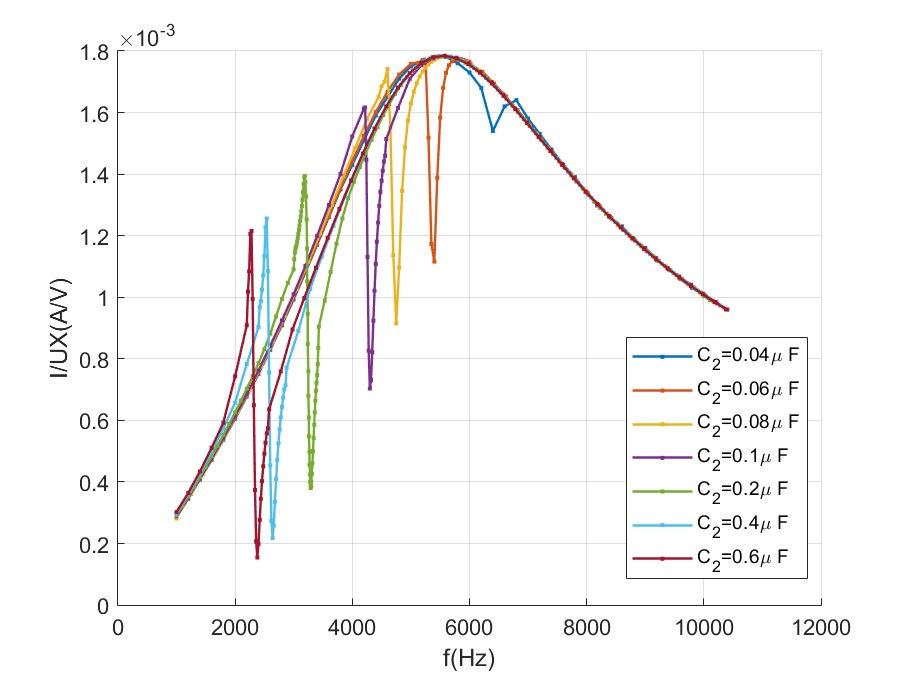
\includegraphics[width=0.5\linewidth]{./figure/Change_C2.jpg}
        \label{fig:7a}
        }
    \subfloat[$\phi -\phi_x$ vs f Graph]{
        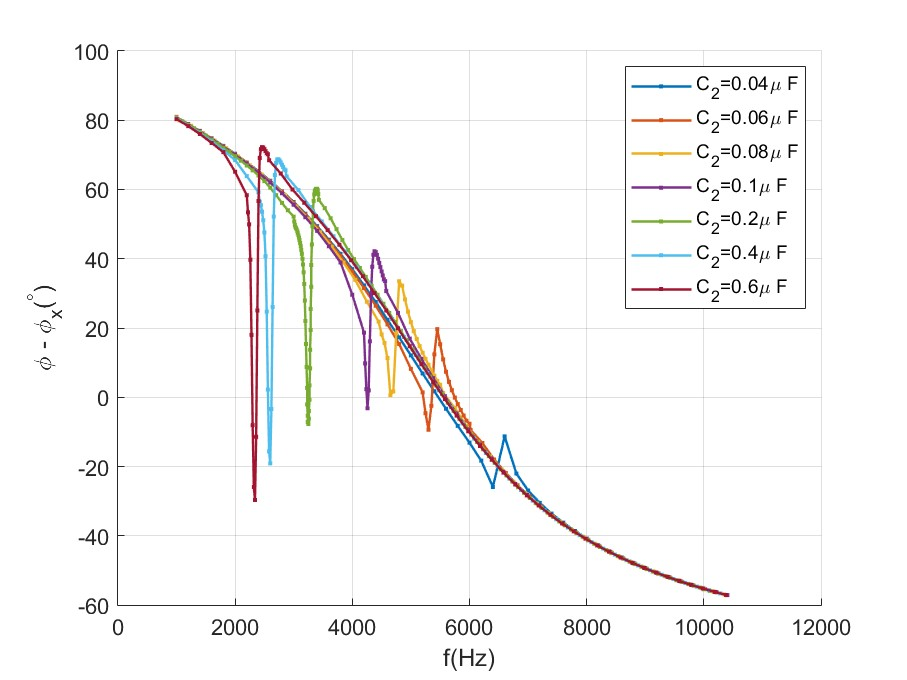
\includegraphics[width=0.5\linewidth]{./figure/phi-phi_x-C_2.jpg}
        \label{fig:7b}
    }
    \caption{不同$C_2$电路中的共振图像}
\end{figure}

由前述理论推导可以得到$C_2$直接影响的参数只有$\omega_2$,其导致的效果是显然的:共振峰右移,幅度明显大于调整$C$的情形。
其峰值的上升也可由前述公式与$\omega_2$的定量关系中给出,相位整体也随$\omega_2$的增大而减小,符合理论预期。
同时我们观察到在$C_2$减小到一定程度时($C_2 = 0.04\mu F$线)图\ref{fig:7a}出现了峰谷反转现象。
为解释这一现象,对$f_1$做一数量级估计可发现其大致处于$\sim 5000$Hz数量级,即为图中最高点处。
当$C_2$较小时$\omega_2$与$\omega_1$的大小顺序发生反转,因此出现了峰谷反转现象。

\section{总结与改进}

除了实验器材方面,主要有以下几个方面需要该进:
\begin{enumerate}
    \item 在稳压二极管的测量中,没有利用LabVIEW中的虚拟测量元件实现测量步长的实时调整和正反向电压。
    可以使用Select元件实现类似计算机语言中if语句的功能,从而对采样方案进行调整。
    \item 在调整参数研究Fano共振特征时,对参数的选取可以再合理一点,在各个区间内都以适当的步长选取三个以上的数据点,比如调整$C_2$时可在$\omega_1$和$\omega_2$存在不同大小关系时分别进行一定数量的采样测量。
    \item 在手动调整采样间距的时候可以适当再密集一些,同时在振幅发生明显转折处需要极高的采样率,否则就会出现上文各图中连线不太平滑的数据点组。
    \item 将实验电路图\ref{fig:3}中的电容换成一组互感线圈,如图\ref{fig:8}所示,在参数恰当时也能观察到Fano共振现象,更多细节不在本实验报告中描述。
\end{enumerate}

\begin{figure}[!t]
    \centering
    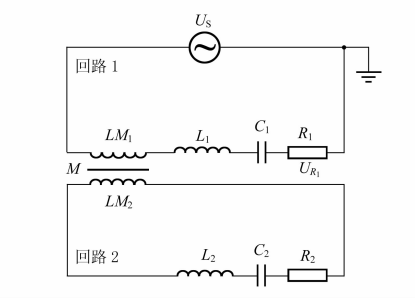
\includegraphics[width=0.5\linewidth]{./figure/互感Fano共振.png}
    \caption{观察Fano共振现象的耦合谐振电路}
    \label{fig:8}
\end{figure}

\begin{thebibliography}{1}
  \bibitem{1} Joe Y S, Satanin A M, Kim C S. Classical analogy of Fano resonances[J]. Physica Scripta, 2006, 74(2): 259.廖慧敏,田广,李智.耦合谐振电路系统中的Fano共振现象[J].物理实验,2022,42(12):10-16.DOI:10.19655/j.cnki.1005-4642.2022.12.002. 
  \bibitem{2} Limonov M F, Rybin M V, Poddubny A N, et al. Fano resonances in photonics[J]. Nature photonics, 2017, 11(9): 543-554.
  \bibitem{3} 廖慧敏,田广,李智.耦合谐振电路系统中的Fano共振现象[J].物理实验,2022,42(12):10-16.DOI:10.19655/j.cnki.1005-4642.2022.12.002. 
\end{thebibliography}

\printbibliography[title={参考文献}]

\end{document}